%sample file for Modelica 2011 Conference paper

\documentclass[11pt,a4paper,twocolumn]{article}
\usepackage{graphicx}
\usepackage{hyperref}
\usepackage{caption}
\usepackage{subcaption}
\usepackage{perpage}
\usepackage{multirow}
\usepackage{pbox}
\usepackage{fixfoot}
\usepackage{epstopdf}
\usepackage{amsmath}
\usepackage{verbatim}

\newcommand{\degree}{\ensuremath{^\circ}}
\MakePerPage{footnote}
% uncomment according to your operating system:
% ------------------------------------------------
\usepackage[latin1]{inputenc}    %% european characters can be used (Windows, old Linux)
%\usepackage[utf8]{inputenc}     %% european characters can be used (Linux)
%\usepackage[applemac]{inputenc} %% european characters can be used (Mac OS)
% ------------------------------------------------
\usepackage[T1]{fontenc}   %% get hyphenation and accented letters right
\usepackage{mathptmx}      %% use fitting times fonts also in formulas
% do not change these lines:
\pagestyle{empty}                %% no page numbers!
\usepackage{geometry}            %% please don't change geometry settings!
\geometry{left=20mm, right=20mm, top=25mm, bottom=25mm, noheadfoot}

\newcommand{\imagedirectory}[1]{../images/{#1}}

% begin the document
\begin{document}
\thispagestyle{empty}

\title{\textbf{Modelica Model for the youBot Manipulator}}
\author{Rhama Dwiputra \quad Alexey Zakharov \quad Roustiam Chakirov \quad Erwin Prassler\\
Bonn-Rhein-Sieg University of Applied Sciences, Department of Computer Science\\
Grantham-Allee 20, 53757 Sankt Augustin}
\date{} % <--- leave date empty
\maketitle\thispagestyle{empty} %% <-- you need this for the first page

\abstract{ 
This paper presents the development of Modelica model for the youBot manipulator.
Whereas other robotic simulations focus on the robot interaction with its environment, Modelica allows the modeling of the manipulator controllers and motors.
The model was developed with a Modelica library for the manipulator's components which provides modularity, reusability and abstraction.
A comparison test with the actual system is performed to ensure the model accuracy.
The test result shows promising result and provides possible future work.
The Modelica model of the youBot manipulator is freely available.
}

\emph{Keywords: Control; Manipulator; Modelica; youBot}

\section{Introduction}
\label{sec:introduction}

\DeclareFixedFootnote{\youbot-store}{\href{http://www.youbot-store.com}{www.youbot-store.com}}
Models and simulation tools are crucial in robotic research. 
Although there have been major improvements in the electronic and mechanical field, robots are still expensive equipments. 
The use of models and simulation tools overcome this problem.
Models and simulation tools allow researchers and university students to experiment with different robots. 
Furthermore, experimentation with models is cost-efficient and time-efficient due to its ability to be automated, conditioned and accelerated.

The \emph{youBot} is a mobile manipulator designed to serve as the reference platform for industry, research and education \cite{Bischoff2011}.
%Similar to Fraunhofer IPAs Care-O-bot\textregistered \cite{Graf2009} and Willow Garages PR2 \cite{Bohren2011}.
%In practice, the youBot has been equipped with an additional laser scanner or 3D camera sensor.
Due to its frequent use as a test subject for educational purpose or investigation of new methods in research institute, a model of the youBot is highly advantageous. 
Robotic simulation tools which has a model of the youBot are VREP \cite{Freese2010}, We-bots \cite{Michel2004} and Gazebo \cite{Koenig2004}.
Like most robotic simulation software, these software focus on simulating the robot interaction with its surrounding environment (navigation, object manipulation) and have its limitation when simulating the robot's internal components (mechanical, electrical, and control system).
Modeling the robot's internal component requires multi-domain capability such as provided by the Modelica\footnote{\href{https://www.modelica.org
}{www.modelica.org}} description language.
Modelica is a non-proprietary, object-oriented, description language for multi domain modeling.
Modelica is maintained by the non-profit Modelica association.
As such, Modelica is suitable for use in education and research. 
The work in this paper is influenced by the existing manipulator model in the Modelica Standard Library or MSL \cite{Elmqvist1999}.

The youBot standard configuration consists of an omnidirectional mobile platform and a five DOFs manipulator with a two finger gripper.
In this paper, the manipulator model is developed by dividing the system into several smaller components.
The component models are stored in a new Modelica library and categorized in different packages based on its functionality.
This approach enables the user to experiment with the manipulator model on the component level.
\begin{comment}
\begin{figure}[htb]
	\centering
	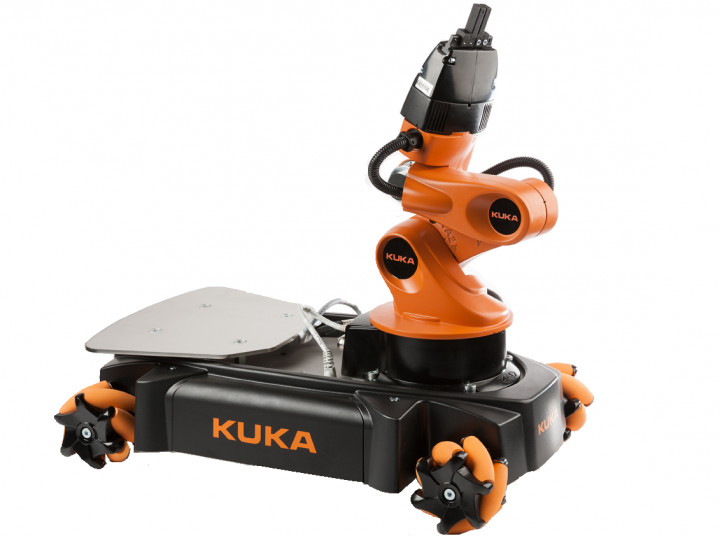
\includegraphics[height=4.4cm]{images/youBot-image.png}
	\caption{Image of youBot\youbot-store}
	\label{fig:youbot}
\end{figure}
\end{comment}

A model is a representation of the actual system and the benefit of having a model only holds true when the model is accurate.
Simulation can result in wrong conclusion when the researcher forget the limitations and condition under which the simulation is valid \cite{Fritzson2004}.
Therefore, the development of the manipulator model is followed by a test with the actual system.
The test compares the behaviors of the actual system and the model throughout a point-to-point motion.
The model accuracy along with the influence of estimated values and approximation is analyzed in the comparison test.

This paper is organized as follows. 
After this introductory section, Modelica related robotic research is presented in Section \ref{sec:state_of_the_art}.
Section \ref{sec:the-youbot-manipulator} presents the specification of the youBot manipulator and Section \ref{sec:the_modelica_package_youbot} describes the Modelica Library for the youBot manipulator. 
Afterward, section \ref{sec:result} presents the evaluation of the developed model.
Finally, section \ref{sec:Conclusion} summarizes the work and provides possible future work.

\section{State of The Art}
\label{sec:state_of_the_art}

Modelica has been used for modeling spider robotic arm \cite{Ferreti2003}, 6-axis industrial robots \cite{Thuemmel2001, Kazi2002, Hast2009}, 3 DOFs parallel Gantry-Tau robot \cite{Dressler2009}, 5 DOFs manipulator \cite{Chen2009} and mobile platforms \cite{Akesson2009, Pohlmann2012}.
In most cases, a robot model in Modelica is used for investigating the  manipulator's motion control especially in the domain of optimization and system dynamics.
Such research requires the repetition of motions and adjustments to the controller which can have damaging effect when being executed on a real robot.

\cite{Kazi2002} performed optimization through iteration to find a compromise between acceleration, velocity and energy consumption and \cite{Hast2009} solved the minimum time optimization problem for an industrial robot.
\cite{Thuemmel2001} derives the inverse dynamic model of a manipulator using algorithms for differential-algebraic equation available in the Dymola\footnote{\href{http://www.3ds.com/products-services/catia/portfolio/dymola}{www.3ds.com/products-services/catia/portfolio/dymola}} software. 
Dymola was also used in \cite{Chen2009} to design a picking manipulator for agriculture purposes.
\cite{Dressler2009} develops method for kinematic calibration with the Modelica model of parallel Gantry-Tau robot.
Aside in the field of motion control, Modelica robot models have also been used for tele-manipulation \cite{Ferreti2003}, robot communication \cite{Pohlmann2012} and teaching tools \cite{Akesson2009}.

As shown from the work presented in this section, there is a wide range of research with robot models in Modelica.
The Modelica model of the youBot manipulator will enable such research to be performed.
Since the youBot is designed to be the reference platform for academic institute, a Modelica model of the youBot manipulator is of high importance.


\section{The youBot Manipulator}
\label{sec:the-youbot-manipulator}
The specification of the manipulator is acquired from the following sources:
\begin{itemize}
\item official youBot website\footnote{\href{www.youbot-store.com}{http://youbot-store.com/
}}, 
\item email communication with the official distributor of the youBot\footnote{\href{info@locomotec.com
}{info@locomotec.com}} and 
\item discussion with researchers from BRICS\footnote{\href{www.best-of-robotics.org}{http://www.best-of-robotics.org/}} who were involved in the development of the youBot's software.
\end{itemize}
This section consist of two subsections, \emph{kinematic chain} and \emph{control system}.
Due to the nature of the robot which is actively being developed, the description presented is subject to changes.


\subsection{Kinematic chain}
\label{ss:kinematic-chain}

The youBot manipulator is a serial chain manipulator with five revolute joints (shown in Figure \ref{fig:youbot-manipulator-real-joints}).
The manipulator is equipped with a two-finger gripper as its end-effector and each finger weights 0.01 kg. 
The fingers' body, position and motion has insignificant influence to the system dynamic when compared to the overall manipulator system.
Therefore, the gripper is modeled only for the visualization purpose.

\begin{figure}[htb]
	\centering
	\includegraphics[height=4.5cm]{\imagedirectory{youbot-manipulator-real-joints.jpg}}
	\caption{The youBot manipulator}
	\label{fig:youbot-manipulator-real-joints}
\end{figure}

The manipulator is 65.5 cm high when fully extended, weights 6.3 kg and has a payload of 0.5 kg.
Each joint is actuated by brushless DC motors and gearboxes with different specifications.
The kinematic chain, joint ranges and dynamic properties of the manipulator are presented in appendix \ref{app:manipulator-specification}.

\subsection{Control System}
\label{ssec:control-system}
The control system accommodates position, velocity and current control in each joint. 
For each joint, the control system consists of: 1. three cascaded \emph{proportional-integral-derivative} or PID controllers, 2. a velocity ramp or v-ramp generator and 3. a space vector pulse width modulation (SVPWM).
Two modes are available for joint position control, \emph{PID} and \emph{v-ramp} mode.
The PID mode calculates the joint velocity in a PID controller whereas in the v-ramp mode, a trapezoidal velocity profile will be generated by the v-ramp generator for the joint velocity.
In this paper, the developed model is based on the joint position control in PID mode.
Figure \ref{fig:controller-overview} shows the overview of the manipulator's controller.
\begin{figure}[htb]
	\centering
	\includegraphics[width=7.6cm]{\imagedirectory{controllerOverview}}
	\caption{Controller overview}
	\label{fig:controller-overview}
\end{figure}

Where $\theta$ is the joint angle, $v$ is the joint velocity and $i$ is the motor current.
The \emph{set} variables ($\theta_{set}$, $v_{set}$, $i_{set}$) are the input values for the PID, the \emph{actual} variables are the values from the manipulator's sensors and the \emph{input} variables are the user defined values.
When controlling the joint position, a user provides the $\theta_{input}$ for the controller and the \emph{Velocity PID} receive the output of the \emph{Position PID} as its $v_{set}$.
When controlling the joint velocity, a user provide the $v_{input}$ for the controller which is directly forwarded as $v_{set}$ to the \emph{Velocity PID} (the output of the \emph{Position PID} in such cases will be ignored).
The \emph{Position PID} is replaced with the v-ramp generator in v-ramp mode.
The PID controllers for position, velocity and current have similar architecture.
As a representative of the PID controllers, Figure \ref{fig:velocity-PID-controller} shows the overview of the PID controller for velocity (\emph{Velocity PID}).
\begin{figure}[htb]
	\centering
	\includegraphics[width=8.2cm]{\imagedirectory{velocityPIDOverview}}
	\caption{Velocity PID overview}
	\label{fig:velocity-PID-controller}
\end{figure}

Where $e$ is the difference between the set value and the actual value. $K_{p}$, $K_ {i}$, and $K_{d}$ are the gain parameters for the controllers.
The output of the \emph{Velocity PID} is forwarded to the \emph{Current PID} as $i_{set}$.
As observed in Figure \ref{fig:velocity-PID-controller}, the Velocity PID controller is similar to the text book PID as follows:
\begin{equation}
\label{eq:textbookpid}
C = K_{p}e(t) + K_{i}\int_{t-\Delta{t}}^{t}e(t)dt + K_{d}\frac{d}{dt}e(t)
\end{equation}
Where $C$ is the controller output and $\Delta t$ is the PID period.
However, the gain parameter in the velocity PID adjusts itself based on the motor velocity as follows:
\begin{equation}\label{eq:gain2-2} 
 k =  \left\{
	 \begin{array}{l l}
    k_{2} & \quad \text{if $\left| v \right| \geq a$}\\
    k_{1} + (\frac{\left| v \right|}{a} * (k_{2} - k_{1}) )  & \quad \text{if $\left| v \right| < a$}
\end{array} \right. 
\end{equation} 
Where $k$ is the gain parameters ($K_{p}$, $K_ {i}$ or $K_{d}$ in Equation \ref{eq:textbookpid}), $k_{1}$ is the lower boundary of the gain parameter, and $k_{2}$ is the upper boundary of the gain parameter value, $v$ is the motor velocity and $a$ is the threshold value for the motor velocity. 
The \emph{Position PID} has the same characteristic as the \emph{Velocity PID}.
Therefore, the \emph{Position PID} and the \emph{Velocity PID} are referred as the non-linear PID.
The non-linear PID enables the user to set different control behaviors for low and high velocity.
Similar to the gain parameters, limiters in the position and velocity controller have non-linear characteristic where the limit value is defined by the motor velocity.

\begin{comment}
In the case of v-ramp mode, the position PID will be disabled and the set velocity is produced by v-ramp generator.
The \emph{textbook} PID controller calculates its output as follows:
\begin{equation}
\label{eq:textbookpid}
C = K_{p}e(t) + K_{i}\int_{t-\Delta{t}}^{t}e(t)dt + K_{d}\frac{d}{dt}e(t)
\end{equation}
\end{comment}


\begin{comment}
\subsubsection{Velocity Ramp Generator}
The velocity ramp or v-ramp generator is used to generate a trapezoidal velocity profile for point-to-point motion.
Figure \ref{fig:vramp-generator-motion-profile} shows the resulting position and acceleration profile from the trapezoidal velocity profile where $s$ is the distance traveled, $v$ is the velocity and $a$ is the acceleration.
\begin{figure}[htb]
	\centering
	\includegraphics[width=8cm]{\imagedirectory{motion_profileVRAMP}}\\
	\caption{V-ramp generator motion profile}
	\label{fig:vramp-generator-motion-profile}
\end{figure}
There are several ways to produce a trapezoidal velocity profile (in theory and practice).
\end{comment}



\section{The \emph{youBot} Modelica Library}
\label{sec:the_modelica_package_youbot}
The Modelica library for the youBot manipulator in this paper is developed with Dymola.
The library is developed using a ``divide and conquer'' principle with emphasize on modularity, re-usability and abstraction.
This approach enables components exchange and component-based experiment.
Additionally, a template model is provided for components which are frequently used in the manipulator model.
In such cases, the model has adjustable parameter sets to be configured based on its implementation.
Finally, the manipulator model is developed in different abstraction layers (Figure \ref{fig:abstraction-layers}).
The lower layer provides a more detailed information in each component and the upper layer provides the general overview of the system.
%Through inheritance, the selected parameter sets of the component in the lower level can be configured from the upper level.

\begin{figure}[htb]
	\centering
	\includegraphics[height=2.4 cm]{\imagedirectory{AbstractionLayer}}
	\caption{Abstraction layer in a manipulator model}
	\label{fig:abstraction-layers}
\end{figure}

In every modeling process, using estimated values and approximation is unavoidable mainly due to the following reasons:
\begin{itemize}
%\item \emph{Computational load}. 
%The computational load of a model is proportional to the model's complexity. 
%Complex component can be approximated with a simple model under the condition that the model accuracy is consistent.
\item \emph{Limited knowledge}. 
Many parameter set of a dynamic system are estimated through system identification (friction, inertia tensor).
\item \emph{Restricted information}. 
Many manufactures do not provide complete information about their product.
\end{itemize}
The use of estimated values and approximation is presented in the description of each package.
The youBot Modelica library consists of four packages which are:
\begin{itemize} 
	\item \emph{Controller} package, 
	\item \emph{Axis} package, 
	\item \emph{Body} package and 
	\item \emph{System} package.
\end{itemize}
The library is developed with the use of several packages in MSL such as Modelica.Blocks.Math for standard mathematical functions and Modelica.Mechanics for 3-dimensional mechanical systems.
This paper follows the Modelica convention in describing the models.
Model's name or package's name begins with capital letter.
When necessary, the model includes its package name. 
The model $Modelica.Blocks.Interfaces.RealInput$ refers to the model \emph{RealInput} which is inside the package \emph{Interfaces}. 
The Interfaces package is inside the \emph{Blocks} package and the $Blocks$ package is inside the MSL.
An instance of a model is written in lower case aside from a few exceptional cases (e.g. \emph{V} is used for voltage to differentiate from \emph{v} for velocity).
\subsection{\emph{Controller} Package}
\label{ssec:controller_package}
The $Controller$ package consists of the components for the manipulator control system.
The $Controller$ package is divided into three packages which are the \emph{Components} package, the \emph{PIDs} package and the \emph{Modes} package.
The $Controller.Components$ package consists of models which are in the lowest level of abstraction layer.
Figure \ref{fig:model-components} show the models in the \emph{Controller.Component} package. 
\begin{figure}[htb]
	\vspace{0.2cm}
	\begin{subfigure}[htb]{0.11\textwidth}
	\centering
	\includegraphics[height=1.6cm]{\imagedirectory{limiter2.png}}
	\caption{$Limiter2$}
	\label{fig:limiter2}
	\end{subfigure}
	\begin{subfigure}[htb]{0.11\textwidth}
	\centering
	\includegraphics[height=1.6cm]{\imagedirectory{gain2.png}}
	\caption{$Gain2$}
	\label{fig:gain2}
	\end{subfigure}
	\begin{subfigure}[htb]{0.11\textwidth}
	\centering
	\includegraphics[height=1.6cm]{\imagedirectory{DisDer.png}}
	\caption{$DisDer$}
	\label{fig:disder}
	\end{subfigure}
	\begin{subfigure}[htb]{0.11\textwidth}
	\centering
	\includegraphics[height=1.6cm]{\imagedirectory{p2v.png}}
	\caption{$P2V$}
	\label{fig:p2v}
	\end{subfigure}
	\caption{The $Controller.Component$ models}
	\label{fig:model-components}
\end{figure}

Following the Modelica convention, the instance's name of a model is placed on the upper part of the symbols in blue color.
The model \emph{Limiter2} and \emph{Gain2} (Figure \ref{fig:gain2} and \ref{fig:limiter2}) perform the calculation for non-linear PID controller (Equation \ref{eq:gain2-2}).
The model \emph{DisDer} (Figure \ref{fig:disder}) produces the derivative value of a specific time period from a discretized continuous input. The model \emph{P2V} (Figure \ref{fig:p2v}) converts PWM rate to voltage rate. The \emph{P2V} model is an approximation of the SVPWM component in the controller.

The \emph{Controller.PIDs} package consists of three different PID models which are the \emph{Position}, \emph{Velocity} and the \emph{Current} model. As the name suggests, the models are the PID controllers for position, velocity and current in the youBot manipulator (Figure \ref{fig:controller-overview}). 
As a representative, Figure \ref{fig:velocity-PID-modelica-model} shows the $PIDs.Velocity$ model.
\begin{figure}[htb]
	\includegraphics[width=8cm]{\imagedirectory{VelocityPID}}
	\caption{$PIDs.Velocity$}
	\label{fig:velocity-PID-modelica-model}
\end{figure}

Where $v\_set$, $v\_actual$ and $i\_set$ represent $v_{set}$, $v_{actual}$ and $i_{set}$ in Figure \ref{fig:velocity-PID-controller} respectively. 
The additional component $N$ in the model produces the output in mA to mimic the readings of the actual system.

Finally, the $Controller.Modes$ package is for different types of control mode. 
Currently, the available model in the $Modes$ package is the \emph{Position} model.
Figure \ref{fig:position-mode-modelica-model} shows the $Modes.Position$ model.
\begin{figure}[htb]
	\includegraphics[width=8cm]{\imagedirectory{PositionMode}}
	\caption{ $Modes.Position$ }
	\label{fig:position-mode-modelica-model}	
\end{figure}

The $Modes.Position$ model consist of all three PID models from the $Controller.PIDs$ package.
$V\_set$ represent the voltage value which will be connected to the motor's power supply unit.
Using the same approach, the model for other control mode explained in Section \ref{ssec:control-system} can also be developed.

\subsection{\emph{Axis} Package}
\label{ssec:axis_package}
The $Axis$ package consists of the model for joint actuator (motor and control system).
The package is named \emph{Axis} because the model will be connected to the rotating axis of the manipulator's joints. 
The $Axis$ package consists of the \emph{Position} model shown in Figure \ref{fig:position-axis-modelica-model}.
\begin{figure}[htb]
	\includegraphics[width=8.3cm]{\imagedirectory{PositionAxis}}
	\vspace{0.2mm}
	\caption{$Axis.Position$}
	\label{fig:position-axis-modelica-model}
\end{figure}

Where $DCPM$ represents the brushless DC motor model, $PSU$ represents the power supply unit model, $R$ represents the gearbox model, $F$ represents the friction model, $controller$ is the $Modes.Position$ model (Figure \ref{fig:position-mode-modelica-model}), $sens\_v$ represent the joint's velocity sensor, $sens\_theta$ represent the joint's position sensor and $joint$ is the connector to the manipulator's joint model.
The $controller$ output ($V\_set$ in Figure \ref{fig:position-mode-modelica-model}) is connected to $PSU$ and its input is extended for the model input as $theta\_set$.
The output of $sens\_v$, $sens\_theta$ and the value of \emph{DCPM}'s current is connected to the control system ($theta\_actual$, $v\_actual$ and $i\_actual$ in Figure \ref{fig:position-mode-modelica-model}).
Aside from the controller, the component in \emph{Modes.Position} are from MSL.

\subsection{\emph{Body} package}
\label{ssec:body_package}

The $Body$ package consists of models for the rigid body model of the manipulator's kinematic chain.
The $Body$ package has three models which are \emph{Gripper}, \emph{Link} and \emph{Manipulator}.
The $Body.Gripper$ model is the rigid body model of the youBot two finger gripper.
Figure \ref{fig:body-gripper-model} shows the $Body.Gripper$ model.
\begin{figure}[htb]
	\centering
	\includegraphics[width=8.2cm]{\imagedirectory{gripper}}
	\vspace{0.2cm}
	\caption{$Body.Gripper$}
	\label{fig:body-gripper-model}
\end{figure}

Where $RF\_rot$ is the gripper's reference frame rotation, $frame\_a$ is the connector to the previous link model, and $gripper$, $left\_finger$ and $right\_finger$  are the rigid body model of the gripper body, left finger and right finger respectively.
$marker$ is a weightless body model to visualize the path of the manipulator's end effector in simulation and $RF\_vis$ provides the visualization of its reference frame.

The $Body.Link$ model is the rigid body model of a manipulator link.  
Figure \ref{fig:link-model} shows the $Body.Link$ model.
\begin{figure}[htb]
	\centering
	\includegraphics[width=7.8cm]{\imagedirectory{Link}}
	\vspace{0.2mm}
	\caption{$Body.Link$}
	\label{fig:link-model}
\end{figure}

Where $joint$ represent the link's joint which is connected to the actuator model through the connector $motor$, $frame\_b$ is the connector to the next link model and the $body$ represent the rigid body of the link.
$frame\_a$, $RF\_rot$ and $RF\_vis$ represent the same components as in $Body.Gripper$ model.

The $Body.Manipulator$ model represent the rigid body model of the youBot manipulator's kinematic link.
Figure \ref{fig:body-manipulator-model} shows the $Body.Manipulator$ model.
\begin{figure}[htb]
	\centering
	\includegraphics[width=7.5cm]{\imagedirectory{Manipulator}}
	\caption{$Body.Manipulator$}
	\label{fig:body-manipulator-model}
\end{figure}

Where $link1$ represent the first link of the manipulator ($Body.Link$, Figure \ref{fig:link-model}), $gripper$ is the manipulator's gripper model ($Body.Gripper$, Figure \ref{fig:body-gripper-model}), $base$ represent the rigid body of the manipulator's base. The component $base\_pos$ is for defining the manipulator position in the world reference frame. 
The $Body.Manipulator$ model has five connectors ($axis1$ to $axis5$) for each joint model and one connector ($world\_rf$) for the world reference frame.



\subsection{\emph{System} package}
\label{ssec:system_package}
The $System$ package consists of the manipulator ready-to-use models.
The $System$ package has two models which are the \emph{Position} model and the \emph{Dummy} model.
The $System.Position$ model is the rigid body model of youBot manipulator's kinematic chain and its actuators.
Figure \ref{fig:modelica-model} shows the $System.Position$ model and its visualization in Dymola whereas Figure \ref{fig:parameter-adjustment} shows the parameter set configuration for the velocity controller in the manipulator's fifth joint.

\begin{figure}[htb]
	\begin{subfigure}[htb]{0.5\textwidth}
	\includegraphics[width=6.5cm]{\imagedirectory{ManipulatorSystem}}
	\caption{$System.Position$}
	\vspace{6mm}
	\label{fig:system-manipulator-model}
	\end{subfigure}		
	\begin{subfigure}[htb]{0.5\textwidth}
	\centering
	\includegraphics[width=5.7cm]{\imagedirectory{Manipulator_Vis}}
	\caption{Model visualization}
	\label{fig:Manipulator_Vis}
	\end{subfigure}		
	\caption{The youBot manipulator model}
	\label{fig:modelica-model}	
\end{figure}

\begin{figure}[htb]
	\centering
	\includegraphics[width=8.1cm]{\imagedirectory{axis_5_parameters}}
	\caption{Parameters configuration}
	\label{fig:parameter-adjustment}	
\end{figure}

In Figure \ref{fig:system-manipulator-model}, $KL$ represents the rigid body model of the youBot manipulator's kinematic chain, $theta\_5$ represents the user defined joint angle and $axis\_5$ represents the actuator (Figure \ref{fig:position-axis-modelica-model}) for joint 5.
The parameter names in Figure \ref{fig:parameter-adjustment} are consistent with the existing driver and firmware.
The $System.Dummy$ model is the rigid body model of the youBot manipulator (\emph{Body.Manipulator}, Figure \ref{fig:body-manipulator-model}) connected to dummy actuators ($Modelica.Mechanics.Rotational.Speed$).
The user can set the velocity of each joint directly in the $System.Dummy$ model.
The $System.Dummy$ model is used for comparison test in Section \ref{sec:result}.






\section{Comparison Test}
\label{sec:result}

A comparison test with the actual system is performed after the development of the manipulator model.
The test purpose is to evaluate the model accuracy and identify the major components which require further development.
The test involves the comparison of the joint position and the joint velocity throughout a point-to-point motion.
For the actual system, the joint velocity is recorded while performing the motion.
The sensor measurement of the joint velocity is assumed to be accurate.
Afterward, the recorded joint velocity is used as input for the System.Dummy model.
In the same setting, the manipulator model ($System.Position$, Figure \ref{fig:system-manipulator-model}) is also performing the same motion.

\begin{figure}[htb]
	\begin{subfigure}[htb]{0.5\textwidth}
	\centering
	\includegraphics[width=6.8cm]{\imagedirectory{EvaluationComparisonVisualNew}}
	\vspace{0.6cm}
	\caption{Error Visualization}
	\vspace{0.4cm}
	\label{fig:error-visualization}
	\end{subfigure}
	\begin{subfigure}[htb]{0.5\textwidth}
	\includegraphics[width=8.2cm]{\imagedirectory{EvaluationErrorJointAngles}}
	\caption{Joint angle difference}
	\label{fig:error-joint-angle}
	\end{subfigure}
	\caption{Test result}
	\label{fig:test-result}
\end{figure}


The manipulator's joints in this test are set to be frictionless.
The motion involves all joints moving 90$^\circ$.
Such motion was chosen so that the resulting error will be the accumulation of the estimated value and approximation in all joints.
Figure \ref{fig:error-visualization} shows the end-effector paths during the motion (the gray-colored youBot manipulator is the starting pose of the motion.) whereas Figure \ref{fig:error-joint-angle} shows the error in joint position.
As expected, the path generated by the model is smoother than that of the actual system as a result of the idealistic conditions in the simulation.
The sum of error from all joint peaked at the value of 0.55 radian.
The error in each joint depends on the maximum velocity parameter ($v_{max}$) in the controller.
As shown in Figure \ref{fig:error-joint-angle}, joint 3 ($v_{max}=4.19$ rad $\cdot$ s$^{-1}$) has a considerably lower peak than joint 5  ($v_{max}=5.90$ rad $\cdot$ s$^{-1} $).
The error in joint angle peaked at two points.
Both peak points happened slightly after the velocity change (from stop to move and slowing down from a constant velocity).
This is consistent with the error in joint velocity as shown in Figure \ref{fig:joint-velocity-comparison}.

\begin{figure}[htb]
	\begin{subfigure}[htb]{0.5\textwidth}
	\centering
	\includegraphics[width=8.2cm]{\imagedirectory{EvaluationJoint3}}
	\vspace{3mm}
	\caption{Joint 3}
	\label{fig:EvaluationJoint3}
	\end{subfigure}		
	\begin{subfigure}[htb]{0.5\textwidth}
	\centering
	\includegraphics[width=8.2cm]{\imagedirectory{EvaluationJoint5}}
	\vspace{3mm}
	\caption{Joint 5}
	\label{fig:EvaluationJoint5}	
	\end{subfigure}
	\caption{Joint velocity comparison}
	\label{fig:joint-velocity-comparison}	
\end{figure}


The joint velocity in the actual system is less stable than in the simulation (Figure \ref{fig:EvaluationJoint3}).
This is the result of the motor vibration which is excluded from the manipulator model.
The ideal motor model results in the deviation on higher velocity (Figure \ref{fig:EvaluationJoint5}) which correspond to the higher error in joint position for joints with higher $v_{max}$ value in its controller.
Similar phenomena in joint velocity and joint position are also found in other joints.
%From this result, it is concluded that the motor model is the major factor of the deviation. 
Other possible contributing aspects in the deviation between the model and the actual system are the inertia tensor estimation, gearbox elasticity/damping, SVPWM approximation and frictionless joints.



\section{Conclusion}
\label{sec:Conclusion}
In this paper, the development of Modelica model for the youBot manipulator is presented.
The Modelica library for the manipulator components provides the user with modularity, reusability and abstraction.
The model accuracy has been evaluated through a comparison test with the actual system.
The test result shows that the model reflects the actual system within a reasonable deviation. 
Possible improvements for the developed Modelica library is the development of a more accurate motor model and a more comprehensive evaluation of the manipulator component (controller components, power consumption and dynamic properties of every rigid body model).
The manipulator model is planned to be tested with other Modelica tools (OpenModelica, jModelica) and used for hardware-in-the-loop experiments.
The development or design of other manipulator models is also possible through the reusability of the components model in the Modelica library.
The library is publicly available\youbot-store to be used for education or research involving manipulator dynamics, load identification, fault analysis and motion control.

\addcontentsline{toc}{chapter}{References}
\bibliographystyle{ieeetr}
\bibliography{bibtex}

\appendix
\section{Manipulator Specification}
\label{app:manipulator-specification}


\begin{table}[htb]
\begin{scriptsize}
\begin{center}
\caption{Kinematic chain}
\label{tab:youBot-Manipulator-Kinematic-Chain}
\renewcommand{\arraystretch}{1.2}
  \begin{tabular}{| l | c | p{0.5cm} | p{0.5cm} | p{0.5cm} | p{0.5cm} | p{0.5cm} | p{0.5cm} |}
    \hline
    
    \multirow{2}{*}{} & \multirow{2}{*}{\pbox{1cm}{Parent \\ frame}} & \multicolumn{3}{|c|}{Translation ($cm$)}  &  \multicolumn{3}{|c|}{Rotation (degree)} \\ \cline{3-8} 
    & & x & y & z & x & y & z \\ \hline 
    Joint 1 & Base & 2.4 & 0 & 11.5 & 180\degree & 0\degree & 0\degree \\ \hline
    Joint 2 & Joint 1 & 3.3 & 0 & 0 & 90\degree & 0\degree & -90\degree \\ \hline
    Joint 3 & Joint 2 & 15.5 & 0 & 0 & 0\degree & 0\degree & -90\degree \\ \hline
    Joint 4 & Joint 3 & 0 & 13.5 & 0 & 0\degree & 0\degree & 0\degree \\ \hline
    Joint 5 & Joint 4 & 0 & 11.36 & 0 & -90\degree & 0\degree & 0\degree \\ \hline
    Gripper & Joint 5 & 0 & 0 & 5.716 & 90\degree & 0\degree & 180\degree \\ \hline
  \end{tabular}

\vspace{0.5cm}

\caption{Joint range}
\label{tab:youBot-manipulator-joint-range}
\renewcommand{\arraystretch}{1.2}
  \begin{tabular}{| l | c | c | c | c | c |}
    \hline
     & Joint 1 & Joint 2 & Joint 3 & Joint 4 & Joint 5 \\ \hline
    \multirow{2}{*}{Joint range} & -169\degree & -65\degree & -151\degree & -102.5\degree & -165\degree \\ 
	&  169\degree & 90\degree & 146\degree & 102.5\degree & 165\degree \\ \hline
\end{tabular}\\

\vspace{0.5cm}

\caption{Dynamic Properties}
\label{tab:youBot-manipulator-dynamic-property}
\renewcommand{\arraystretch}{1.2}
  \begin{tabular}{| l | c | p{1.1cm} | p{1.1cm} | p{1.1cm} |} \hline
	& \multirow{2}{*}{Mass ($kg$)} & \multicolumn{3}{ |c| }{Intertia Tensor Elements ($kg{\cdot}cm^{2}$)}  \\ \cline{3-5}
     & & $I_{xx}$ & $I_{yy}$  & $I_{zz}$ \\ \hline
     Link 1 & 1.39 & 29.525 & 60.091 & 58.821 \\ \hline
	 Link 2 & 1.318 & 31.145 & 5.483 & 31.631 \\ \hline
	 Link 3 & 0.821 & 17.2767 & 4.1967 & 18.468 \\ \hline
	 Link 4 & 0.769 & 6.764 & 10.573 & 6.61 \\ \hline
	 Link 5 & 0.678 & 1.934 & 1.602 & 0.689 \\ \hline
	 Gripper &  0.201 & 2.324 & 3.629 & 2.067 \\ \hline
  \end{tabular}

\vspace{0.5cm}

\begin{comment}
\caption{Motor \& Gearbox}
\label{tab:youBot-manipulator-motor-gearbox}
\renewcommand{\arraystretch}{1.2}
  \begin{tabular}{| l | c | c | c | c | c |}
    \hline
     & Joint 1 & Joint 2 & Joint 3 & Joint 4 & Joint 5 \\ \hline
    \multicolumn{6}{ |c| }{Motor}  \\ \hline
    Voltage ($V$) & 24 & 24 & 24 & 24 & 24 \\ \hline
    Current ($A$) & 2.36 & 2.36 & 2.36 & 1.07 & 0.49 \\ \hline
   Inductance ($mH$) & 0.573 & 0.573 & 0.573 & 2.24 & 7.73 \\ \hline
   Resistance ($\Omega$) & 0.978 & 0.978 & 0.978 & 4.48 & 13.7 \\ \hline
   Inertia ($kg{\cdot}mm^{2}$) & 13.5 & 13.5 & 13.5 & 9.25 & 3.5 \\ \hline
   Speed ($RPM$) & 5260 & 5260 & 5260 & 2850 & 2800 \\ \hline
   \multicolumn{6}{ |c| }{Gearbox}  \\ \hline
 Ratio & 156 & 156 & 100 & 71 & 71 \\ \hline
\end{tabular}\\
\end{comment}


\end{center}
\end{scriptsize}
\end{table}

\end{document}
